\section{\large Конструкторская часть}

В данном разделе представлены схемы алгоритмов очереди работ и алгоритма шифрования.

\subsection{Очереди работ}

На рисунке \ref{rezat:churok} представлена схема алгоритма очереди работ.

\begin{figure}[ht!]
	\centering{
		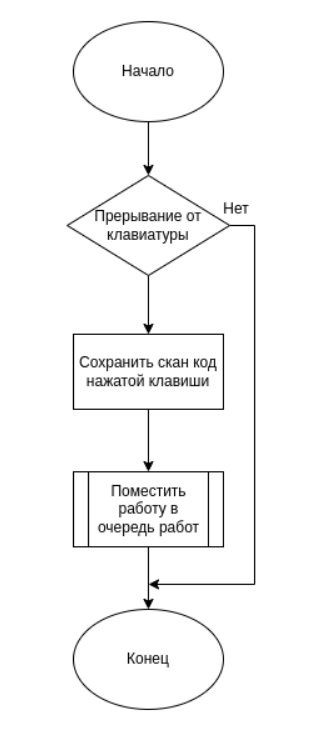
\includegraphics[width=0.3\textwidth]{assets/graphs/workqueue.png}
		\caption{Алгоритм очереди работ}
		\label{rezat:churok}}
\end{figure}

После того как очереди работ считают клавишу с клавиатуры, начинает работать алгоритм шифрования.
На рисунке \ref{vlasov:naydet:menya} представлена схема алгоритма шифрования.

\begin{figure}[ht!]
	\centering{
		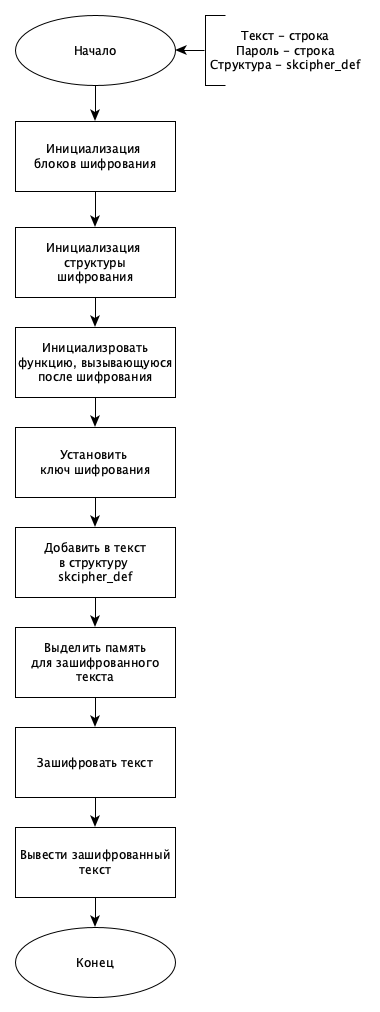
\includegraphics[width=0.5\textwidth]{assets/graphs/cipher.png}
		\caption{Алгоритм шифрования}
		\label{vlasov:naydet:menya}}
\end{figure}

\subsection*{Вывод}

В данном разделе разработаны и представлены схемы алгоритмов очередей работ и алгоритма шифрования.